\documentclass{ucll-slides}

\title{Vlaamse Programmeerwedstrijd}


\setbeamertemplate{title page}{%
  \begin{center}
    {\sc Introductie} \\
    {
      \newlength{\width}
      \settowidth{\width}{\sc Introductie}
      \rule[10pt]{1.4\width}{1pt} \\
    }
    {\sc\huge \inserttitle}
  \end{center}
}

\newcommand{\HERE}[1]{\tikz[remember picture]\node(#1){};}

\begin{document}

\begin{frame}
  \titlepage
\end{frame}

\begin{frame}
  \frametitle{Opzet}
  \begin{center}
    \begin{tikzpicture}[team member/.style={},
                        riddle/.style={}]
      \path[use as bounding box] (-5,0) rectangle (5,-5);

      \node[team member,anchor=south] (rick) at (0,0) {
\includegraphics[height=1cm]{rick.jpg}};
      \node[team member,anchor=south east] at ($ (rick.south west) + (-0.5,0) $) {
\includegraphics[height=1cm]{morty.jpg}};
      \node[team member,anchor=south west] at ($ (rick.south east) + (0.5,0) $) {
\includegraphics[height=1cm]{summer.jpg}};
      \node[fill=blue!25,font=\Large,anchor=north,minimum width=5cm] at (rick.south) {\sc drie teamleden};

      \node[anchor=south] (laptop) at (0,-2.5) {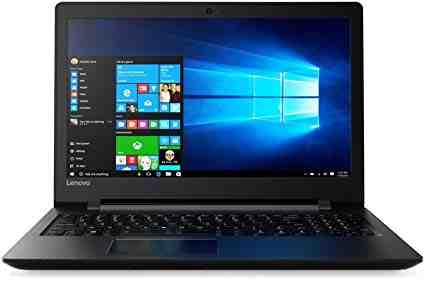
\includegraphics[height=1cm]{laptop.jpg}};
      \node[anchor=north,fill=blue!25,font=\Large,minimum width=5cm] at (laptop.south){\sc \'e\'en laptop};

      \node[riddle,anchor=south] (riddle) at (0,-5) {
\includegraphics[height=1cm]{riddle.jpg}};
      \node[riddle,anchor=south] at (-1,-5) {
\includegraphics[height=1cm]{riddle.jpg}};
      \node[riddle,anchor=south] at (-2,-5) {
\includegraphics[height=1cm]{riddle.jpg}};
      \node[riddle,anchor=south] at (1,-5) {
\includegraphics[height=1cm]{riddle.jpg}};
      \node[riddle,anchor=south] at (2,-5) {
\includegraphics[height=1cm]{riddle.jpg}};
      \node[fill=blue!25,font=\Large,anchor=north,minimum width=5cm] at (riddle.south) {\sc vijf opgaves};

      \begin{scope}[rotate=-20,transform shape,xshift=5cm]
        \node (time) {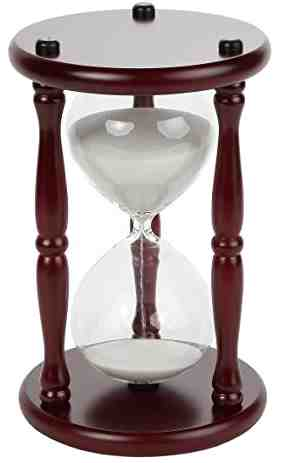
\includegraphics[height=1cm]{hourglass.jpg}};
        \node[anchor=north] at (time.south) {\sc drie uur};
      \end{scope}
    \end{tikzpicture}
  \end{center}
\end{frame}

\begin{frame}
  \frametitle{Opgaves}
  \begin{itemize}
    \item Algoritmisch van aard
          \begin{itemize}
            \item Zie \link{https://www.vlaamseprogrammeerwedstrijd.be/}{offici\"ele pagina} voor opgaves voorbije jaren
            \item Ook beschikbaar op \link{https://github.com/UCLeuvenLimburg/vpw}{GitHub}
          \end{itemize}
    \item Geen Internettoegang
    \item Boeken, offline documentatie, code toegestaan
    \item Vrije keuze programmeertaal
  \end{itemize}
  \begin{center}\small
    \begin{tabular}{cccc}
      C & C++ & C$\sharp$ & Clojure \\[2mm]
      Go & Haskell & Java & Javascript \\[2mm]
      Kotlin & Pascal & Perl & PHP \\[2mm]
      Prolog & Python & Python 3 & Rust \\[2mm]
      Ruby & Scala & Scheme & Visual Basic
    \end{tabular}
  \end{center}
\end{frame}

\begin{frame}
  \frametitle{Categorie\"en}
  \begin{itemize}
    \item Vier moeilijkheidsgraden (categorie\"en)
    \item Toekenning op basis van type opleiding
  \end{itemize}
  \begin{center}
    \begin{tabular}{ll}
      \textbf{Cat-1} & Secundair onderwijs \\[2mm]
      \textbf{Cat-2} & Professionele bachelor\HERE{a} \\[2mm]
      \textbf{Cat-3} & Academische bachelor \\[2mm]
      \textbf{Cat-4} & Al de rest \\
    \end{tabular}
  \end{center}
  \only<2>{
    \begin{tikzpicture}[remember picture,overlay]
      \coordinate (b) at ($ (a) + (0.25,0) $);
      \draw[fill=red] (b) circle [radius=2mm];
      \draw[latex-] (b) -- ($ (b) + (1.25,0.5) $) node[above] {\sc u bevindt zich hier};
    \end{tikzpicture}
  }
\end{frame}

\begin{frame}
  \frametitle{Eerdere Prestaties UCLL Teams}
  \begin{center}
    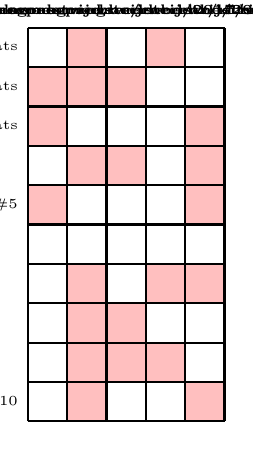
\begin{tikzpicture}
      \path[use as bounding box] (0,0) rectangle (2.5, 5);

      \foreach[count=\i,evaluate={5-\i*0.5+0.25} as \y] \label in {eerste plaats,tweede plaats,derde plaats,,\#5,,,,,\#10} {
        \node[anchor=east,font=\tiny] at (0,\y) {\label};
      }
      
      \foreach[count=\i,evaluate={\i / 2 - 0.25} as \x] \year/\url in {2018/{https://www.vlaamseprogrammeerwedstrijd.be/current/uitslag/Cat-2.html},2017/{https://www.vlaamseprogrammeerwedstrijd.be/2017/uitslag/Cat-2.html},2016/{https://www.vlaamseprogrammeerwedstrijd.be/2016/uitslag/Cat-2.html},2015/{https://www.vlaamseprogrammeerwedstrijd.be/2015/uitslag/Cat-2.html},2014/{https://www.vlaamseprogrammeerwedstrijd.be/2014/uitslag/Cat-2.html}} {
        \node[font={\tiny\bf},anchor=south] at (\x,5) {\link{\url}{\rotatebox{90}{\year}}};
      }

      \foreach[evaluate={2-(\year-2014)/2} as \x,evaluate={5-\rank/2} as \y] \year/\rank in {2018/2,2018/3,2018/5,2017/1,2017/2,2017/4,2017/7,2017/8,2017/9,2017/10,2016/2,2016/4,2016/8,2016/9,2015/1,2015/7,2015/9,2014/3,2014/4,2014/5,2014/7,2014/10} {
        \draw[fill=red!25] (\x,\y) rectangle ++(0.5,+0.5);
      }

      \draw[thick] (0,0) grid[step=5mm] (2.5, 5);

      \node at (1.25,-1) {Rood vakje = winnend UCLL team};
    \end{tikzpicture}
  \end{center}
\end{frame}

\begin{frame}
  \frametitle{Oefenavond}
  \begin{itemize}
    \item Hier op Campus Proximus \\[2mm]
    \item Oplossen oude opgaves \\[2mm]
    \item Bedoeld als kennismaking met VPW \\[2mm]
    \item Casual en optioneel \\[2mm]
    \item Inschrijven op \link{https://ucll-my.sharepoint.com/:x:/g/personal/u0057764_ucll_be/EWnEbNMmJa5CuOZNVRrnky0B6eB_bSX0j4H5jhsJ5Y-ntg?e=PJKN3p}{deze pagina} (kies juiste tab)
    \item Gratis drank en (hopelijk) pizza (Kingslize)
  \end{itemize}
  \vskip5mm
  \begin{center} \Large
    20 februari 2019 vanaf 18:00 \\[2mm]
  \end{center}
\end{frame}

\begin{frame}
  \frametitle{Andere Belangrijke Informatie}
  \structure{Teamvorming}
  \begin{center}
    \link{https://ucll-my.sharepoint.com/:x:/g/personal/u0057764_ucll_be/EWnEbNMmJa5CuOZNVRrnky0B6eB_bSX0j4H5jhsJ5Y-ntg?e=PJKN3p}{Hi-Tech Team Building Assistant Tool}
  \end{center}

  \structure{Deadline Inschrijvingen}
  \begin{center} \Large
    28 februari 2019 om 12:00 \\ \small (\link{https://www.vlaamseprogrammeerwedstrijd.be/current/\#inschrijven}{inschrijvingspagina})
  \end{center}

  \structure{Wedstrijd}
  \begin{center} \Large
    13 maart 2019, 14:00-18:00 \\[2mm]
    AP Hogeschool \\ \large (Antwerpen)
  \end{center}
\end{frame}

\end{document}


%%% Local Variables:
%%% mode: latex
%%% TeX-master:
%%% End:
